\documentclass[11pt]{article}

\usepackage[a4paper,margin=2.4cm]{geometry}
\usepackage[T1]{fontenc}
\usepackage[utf8]{inputenc}
\usepackage{lmodern}
\usepackage{microtype}
\usepackage{graphicx}
\usepackage{booktabs}
\usepackage{amsmath}
\usepackage{siunitx}
\usepackage[round,authoryear]{natbib}
\usepackage[hidelinks]{hyperref}
\usepackage{xcolor}
\usepackage{caption}

\graphicspath{{figures/}}
\captionsetup{font=small,labelfont=bf}
\setlength{\emergencystretch}{2em}
\sisetup{detect-all}
\hypersetup{
  pdftitle={Altitude-Resolved Thermospheric Density Responses, Empirical-Model Residuals, and Secular Trends Across Multiple Long-Record Products},
  pdfauthor={Sergio Gómez Damas}
}

\title{Altitude-Resolved Thermospheric Density Responses,\\
Empirical-Model Residuals, and Secular Trends\\
Across Multiple Long-Record Products}
\author{Sergio G\'omez Damas}
\date{Draft manuscript, 31 August 2026}

\begin{document}
\maketitle

\begin{abstract}
Thermospheric neutral density controls satellite drag but varies across solar,
geomagnetic, seasonal, and secular time scales.  We combine a globally averaged
orbit-derived density record, a Mauna Loa vertical subset of the High Accuracy
Satellite Drag Model (HASDM) database, eight TU Delft accelerometer-derived
mission products, three NRLMSIS-family baselines, paired JB2006/JB2008 baselines,
and TIMED/SABER carbon-dioxide cooling.  The analysis is deliberately
figures-first and separates observational or assimilative products from
empirical-model outputs.  Daily mean HASDM log-density correlates strongly with
centered 81-day F10.7 across 175--825 km ($r=0.815$--$0.943$), more moderately
with SABER CO$_2$ cooling ($r=0.656$--$0.664$), and weakly to moderately with Ap
($r=0.293$--$0.373$).  Its bivariate correlation with tropospheric CO$_2$ is
negative ($r=-0.260$ to $-0.132$), but shared trends and autocorrelation preclude
a causal interpretation.  On 9,301 exact common dates, empirical-model errors
show distinct altitude-dependent bias, absolute error, and residual forcing
structure; no model is a universal winner, and calibration overlap limits
independence claims.  After quadratic F10.7 adjustment, median density trends
are $-5.04\%$ decade$^{-1}$ for the global-mean product and
$-6.36\%$ decade$^{-1}$ for the HASDM subset.  Empirical-model baseline trends
range from a median $-0.80\%$ decade$^{-1}$ for JB2006 to
$-11.72\%$ decade$^{-1}$ for JB2008, demonstrating that model-generated trends
are strongly method and forcing dependent.  The results support strong solar
control and negative solar-adjusted trends consistent with contraction in the
observational/reference products,
while showing why pairwise CO$_2$ associations, residual leakage, and empirical
baseline trends must remain descriptive rather than attributional.
\end{abstract}

\section{Introduction}

Neutral density in the thermosphere determines aerodynamic drag on low-Earth
orbiting objects.  Its short- and medium-term variability is dominated by solar
extreme-ultraviolet input and geomagnetic energy deposition, commonly
represented by F10.7 and geomagnetic indices.  On longer time scales, increasing
CO$_2$ enhances infrared cooling in the middle and upper atmosphere and is
expected to contract the thermosphere \citep{roble1989,brown2024}.  Orbit-derived
records consequently show multidecadal density decreases, but trend magnitude
depends on altitude, epoch, solar-cycle treatment, and sampling
\citep{emmert2009,emmert2015,brown2024}.

No single product observes all of the relevant dimensions.  Orbit-derived
global means provide long records but suppress geographic and local-time
structure.  Accelerometer products resolve actual satellite trajectories but
mix mission, altitude, local-time, and epoch effects.  HASDM provides a regular
assimilation-derived density field \citep{storz2005}, while empirical models
such as NRLMSISE-00, NRLMSIS 2.0/2.1, JB2006, and JB2008 encode different
calibration records and forcing proxies \citep{picone2002,emmert2021,emmert2022,
bowman2008jb2006,bowman2008jb2008}.  Comparing these families without preserving
their provenance can turn sampling and model design into apparent physical
differences.

This study asks three linked questions.  First, how does the daily solar
response of mean density and within-day density range vary with altitude and
product?  Second, how do solar, geomagnetic, tropospheric CO$_2$, and SABER CO$_2$
cooling relationships differ between those two density diagnostics?  Third,
what do a strictly paired empirical-model comparison and a common
solar-adjusted trend estimator reveal about model fidelity and long-term
contraction?  Six figures move from coverage and provenance to forcing
relationships, empirical-model residuals, and finally secular trends.  All
correlation and causal-discovery-derived quantities used here are treated as
descriptive diagnostics unless explicitly stated otherwise.

\section{Data and methods}

\subsection{Density products and coverage}

Figure~\ref{fig:coverage} records the available date--altitude support rather
than a scientific response.  The analyzed global-mean artifact spans
1967--2019 at ten altitudes from 250 to 575 km; \citet{emmert2009} describes
the parent orbit-derived product and method, not this artifact's later
extension.  The Mauna
Loa HASDM subset spans 2000--20 July 2025 at 27 levels from 175 to 825 km.  It is
a geographic extraction from an assimilative product, not an in situ density
record.  NRLMSISE-00 and NRLMSIS 2.0/2.1 baselines span 1967--19 April 2026,
and paired JB2006/JB2008 output spans 6 January 1997--19 April 2026, both on
125--825 km grids.  The paired JB record omits 17 May 1998--15 March 1999 because
required provider solar proxies fail the official validity threshold.

The TU Delft version-02 family comprises CHAMP, GOCE, GRACE-A, GRACE-B,
GRACE-FO, and Swarm-A/B/C trajectory products \citep{tudelftdata}.  Their
different altitude and epoch envelopes are retained in Figure~\ref{fig:coverage};
we do not interpret the envelope area as sample density or response strength.
The analyzed TIMED/SABER CO$_2$ cooling artifact covers 2002--2023 over the
available 100--139 km channels; \citet{mlynczak2010} describes the instrument
record and cooling products through its publication epoch.  Figure provenance,
source-file checksums, row
counts, and exact date support are stored in the machine-readable figure
summary distributed with this manuscript.

\begin{figure}[p]
  \centering
  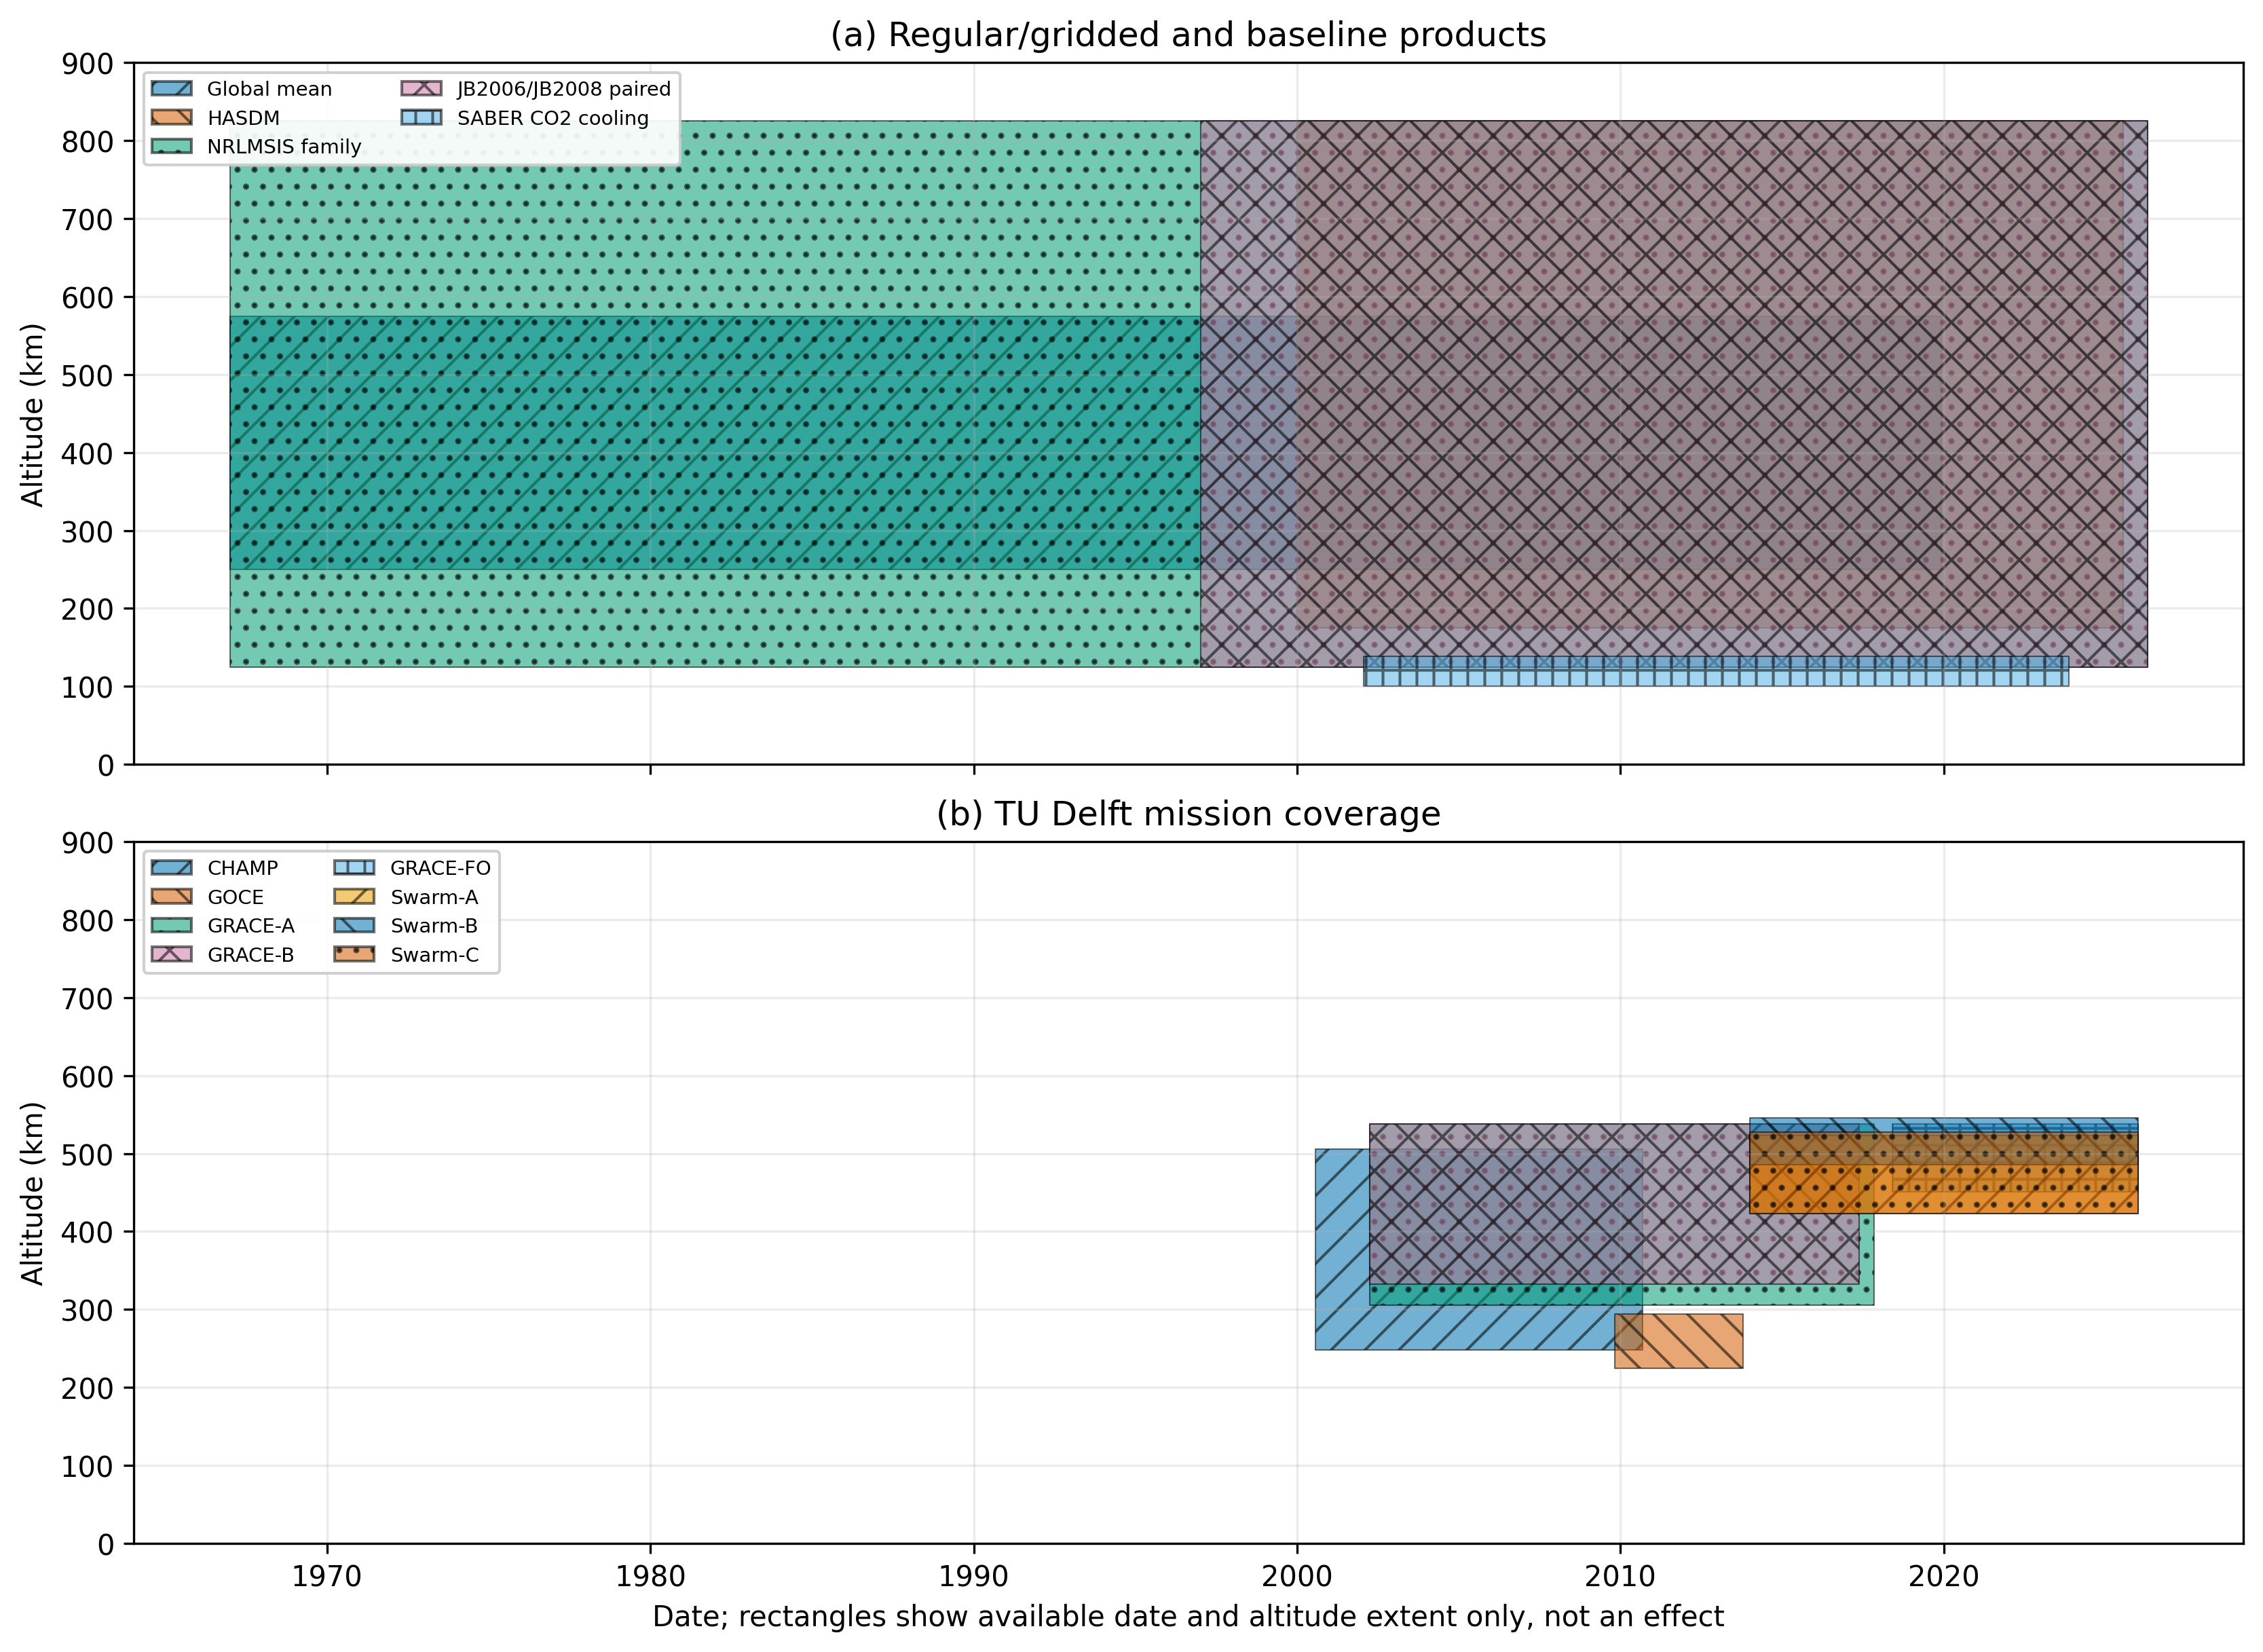
\includegraphics[width=\textwidth]{fig1.pdf}
  \caption{Date--altitude availability for canonical regular/gridded density
  products and each of the eight TU Delft missions.  Rectangle extent denotes
  available records only; it is not evidence of a density response.}
  \label{fig:coverage}
\end{figure}

\subsection{Daily diagnostics and external drivers}

For each gridded altitude, we use the daily mean of $\ell_\rho=\log_{10}\rho$
and the daily within-day range
$\Delta\ell_\rho=\max(\ell_\rho)-\min(\ell_\rho)$.  The solar diagnostic is the
centered 81-day mean of observed F10.7 \citep{tapping2013}; geomagnetic context
is supplied by daily Ap and Kp \citep{matzka2021}.  Tropospheric CO$_2$ is the
NOAA Global Monitoring Laboratory Mauna Loa daily record, including the
provider's documented Maunakea substitution interval \citep{noaaco2}.  SABER
CO$_2$ cooling is averaged daily at the available channel nearest 139 km.

Figures~\ref{fig:response} and \ref{fig:relationships} report pairwise Pearson
correlations and Fisher-transform 95\% intervals after pairwise omission of
missing values.  These intervals are nominal: they do not correct the effective
sample size for serial dependence, and the large daily samples should not be
read as equivalent independent observations.  Figure~\ref{fig:scatter} therefore
shows points without fitted lines.  TU Delft is omitted from
Figure~\ref{fig:response} because a comparable mission-aware daily-altitude
aggregation was not precomputed; inventing one solely for the composite would
confound trajectory sampling with product differences.

\subsection{Paired model error and forcing-fidelity diagnostics}

The empirical-model comparison uses 9,301 exact common dates from 1 January
2000 to 20 July 2025 at all 27 HASDM altitudes.  For model $m$, error is
\begin{equation}
  \epsilon_m(t,z)=\ln\!\left[\frac{\rho_m(t,z)}{\rho_{\mathrm{HASDM}}(t,z)}\right].
\end{equation}
Signed median $\epsilon$ measures multiplicative bias and median
$|\epsilon|$ measures robust absolute error.  Accuracy intervals use 250
deterministic, paired circular calendar-day block-bootstrap replicates with a
27-day block length; each resampled day retains the complete model vector
\citep{kunsch1989}.

Residual forcing fidelity is an exploratory PCMCI+ diagnostic
\citep{runge2020}.  For each model and altitude, residuals and drivers undergo
calendar-day seasonal-anomaly removal, centered three-year rolling-mean
removal, and standardization.  ParCorr PCMCI+ evaluates lags 0--180 days at
$\alpha=0.05$, with majority collider handling, conflict resolution, and
Benjamini--Hochberg false-discovery-rate control within each altitude/run graph
\citep{benjamini1995}.  A plotted nonzero value is the signed partial
correlation at the largest retained absolute effect across lags.  A zero means
that no tested link was retained, not that independence was demonstrated.
Because the single-profile analysis does not establish causal sufficiency,
stationarity across every sensitivity, or invariance across methods, we do not
interpret these links causally.

Model/reference independence also varies.  JB2008 development used Air Force
HASDM, CHAMP, and GRACE density domains; JB2006 used density corrections from a
HASDM-related modelling chain.  NRLMSIS 2.0 used global orbit-derived densities
for fitting but reserved CHAMP and GOCE for comparison, and NRLMSIS 2.1 retained
the 2.0 mass-density formulation while adding NO \citep{emmert2021,emmert2022,
bowman2008jb2006,bowman2008jb2008}.  Thus Figure~\ref{fig:model} is a
HASDM-referenced disagreement and residual-structure comparison, not a wholly
independent validation or a universal model ranking.

\subsection{Solar-adjusted trend estimation}

At each retained altitude, the trend model is
\begin{equation}
\ell_\rho(t)=\beta_t(t-\bar t)+\beta_1(F-\bar F)
 +\beta_2(F-\bar F)^2+\alpha+e(t),
\end{equation}
where $F$ is centered-81-day F10.7.  TU Delft pooled altitude bins additionally
include mission fixed offsets.  A series requires at least 365 finite samples
and an 11-year span.  The log-density time coefficient is transformed to
percent per decade as
\begin{equation}
  100\left(10^{10\beta_t}-1\right).
\end{equation}
Confidence limits separately transform the endpoints of a 95\% interval based
on a 27-calendar-day Bartlett Newey--West heteroskedasticity- and
autocorrelation-consistent covariance estimate \citep{neweywest1987}.

Panel~A of Figure~\ref{fig:trends} is a vector reconstruction of 427
plot-precision values extracted from Figure~2 of \citet{brown2024}, with all 16
study labels and the original $-7$ to $1\%$ decade$^{-1}$ horizontal domain.
The source article is CC BY 4.0.  These digitized curves preserve published
figure geometry but do not replace the original studies' data.  Panel~B applies
the common estimator above.  Its trends are solar-adjusted descriptions, not
CO$_2$-only causal effects.

\section{Results}

\subsection{Coverage constrains every cross-product comparison}

The broadest record is the global-mean product, while HASDM provides the widest
regular altitude span in the common 2000--2025 interval
(Figure~\ref{fig:coverage}).  The NRLMSIS family extends across nearly six
decades because it is model generated.  JB support is shorter and contains a
forcing-availability gap.  TU Delft trajectories occupy narrower,
mission-specific bands: GOCE samples the lowest envelope, GRACE-FO and Swarm-B
the highest, and only a subset of bins spans the 11-year threshold used for
trend estimation.  These differences motivate product-specific sample counts
and prevent a single nominal ``common coverage'' from being assigned to all
figures.

\subsection{Solar response is strong for mean density but changes sign for daily range}

Daily mean log-density is positively correlated with centered-81-day F10.7 for
every regular product (Figure~\ref{fig:response}).  Across altitude, the global
mean has $r=0.892$--$0.930$, HASDM $r=0.815$--$0.943$, NRLMSISE-00
$r=0.289$--$0.952$, NRLMSIS 2.0/2.1 $r=0.307$--$0.951$, JB2006
$r=0.612$--$0.954$, and JB2008 $r=0.656$--$0.900$.  The lower correlations at
the bottom of several empirical profiles and the convergence toward strong
positive correlations aloft show that a model's solar response cannot be
summarized by one altitude-independent coefficient.

The daily-range panel behaves differently.  HASDM spans $r=-0.554$ to $0.899$;
the NRLMSIS products and JB models similarly transition from negative responses
at lower altitudes to positive responses aloft.  This sign reversal concerns
within-day log-density range, not mean density or a negative solar-heating
effect.  It can reflect altitude-dependent composition, local-time structure,
geomagnetic variability, and how each daily gridded product samples those
processes.

\begin{figure}[p]
  \centering
  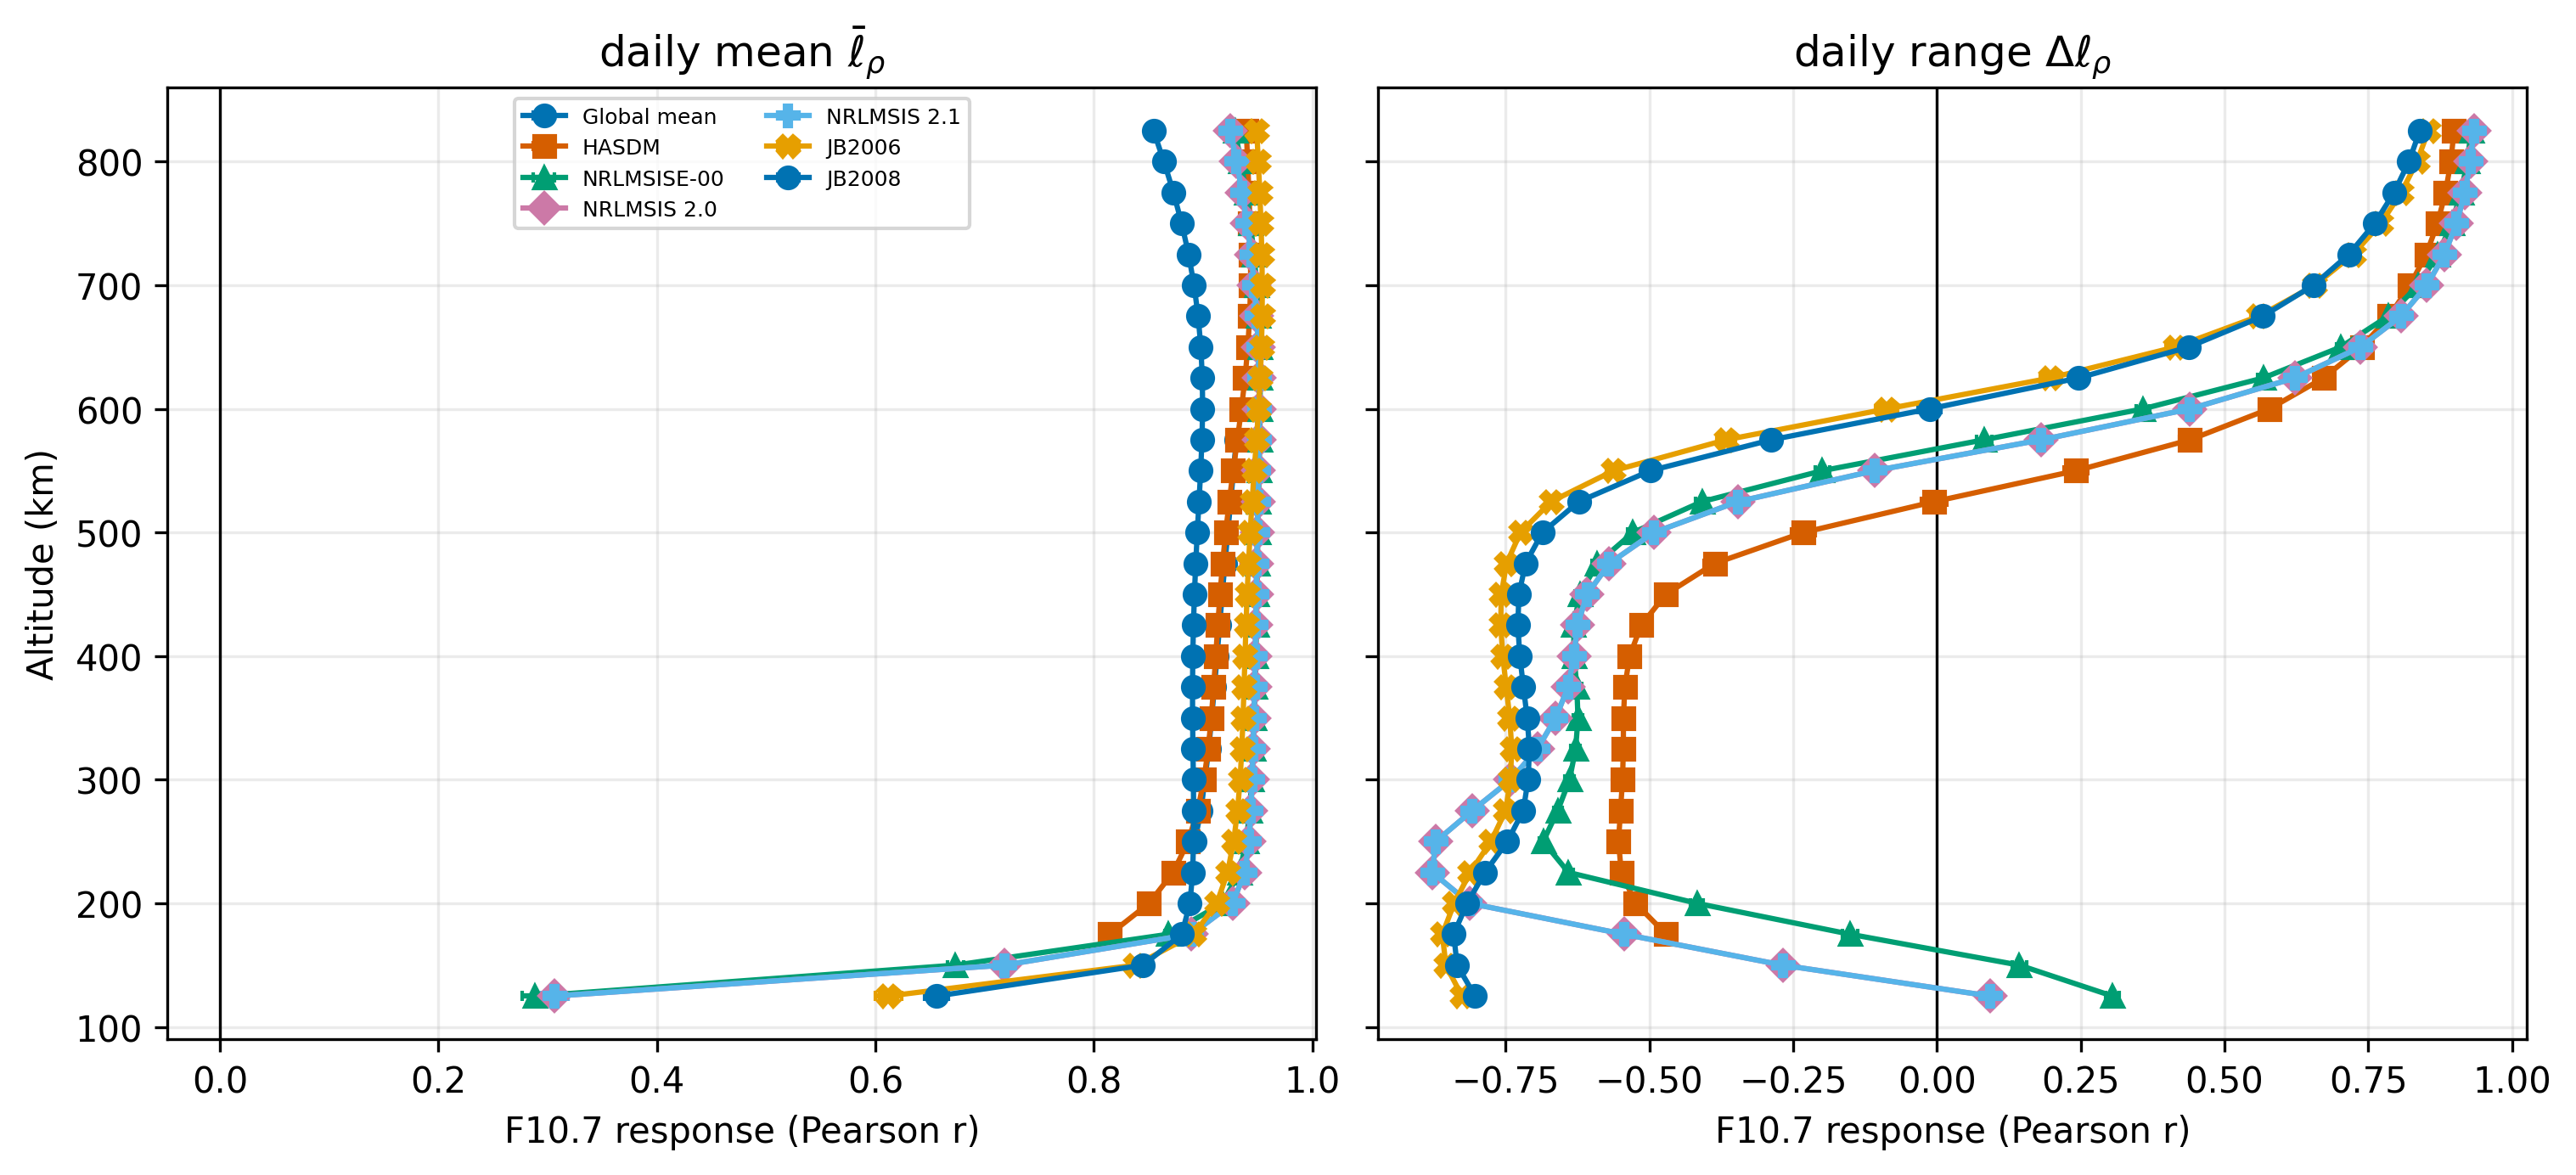
\includegraphics[width=\textwidth]{fig2.pdf}
  \caption{Pearson correlations of centered 81-day F10.7 with daily mean
  log$_{10}$ density and daily within-day log-density range by altitude.
  Horizontal bars are nominal Fisher 95\% intervals; product-specific support
  is retained.  TU Delft is omitted because a comparable mission-aware daily
  aggregation was not precomputed.}
  \label{fig:response}
\end{figure}

\subsection{\texorpdfstring{CO$_2$}{CO2} and SABER cooling associations remain descriptive}

The scatter matrix in Figure~\ref{fig:scatter} exposes the joint distribution,
outliers, and heteroscedasticity hidden by an altitude-profile summary.  Each
non-SABER pair has 7,959 complete days and each SABER pair 7,915 days.  Mean
density visibly follows the solar cycle at both 175 and 825 km.  Relationships
for daily range differ strongly between those endpoints, consistent with the
sign changes in Figure~\ref{fig:response}.

\begin{figure}[p]
  \centering
  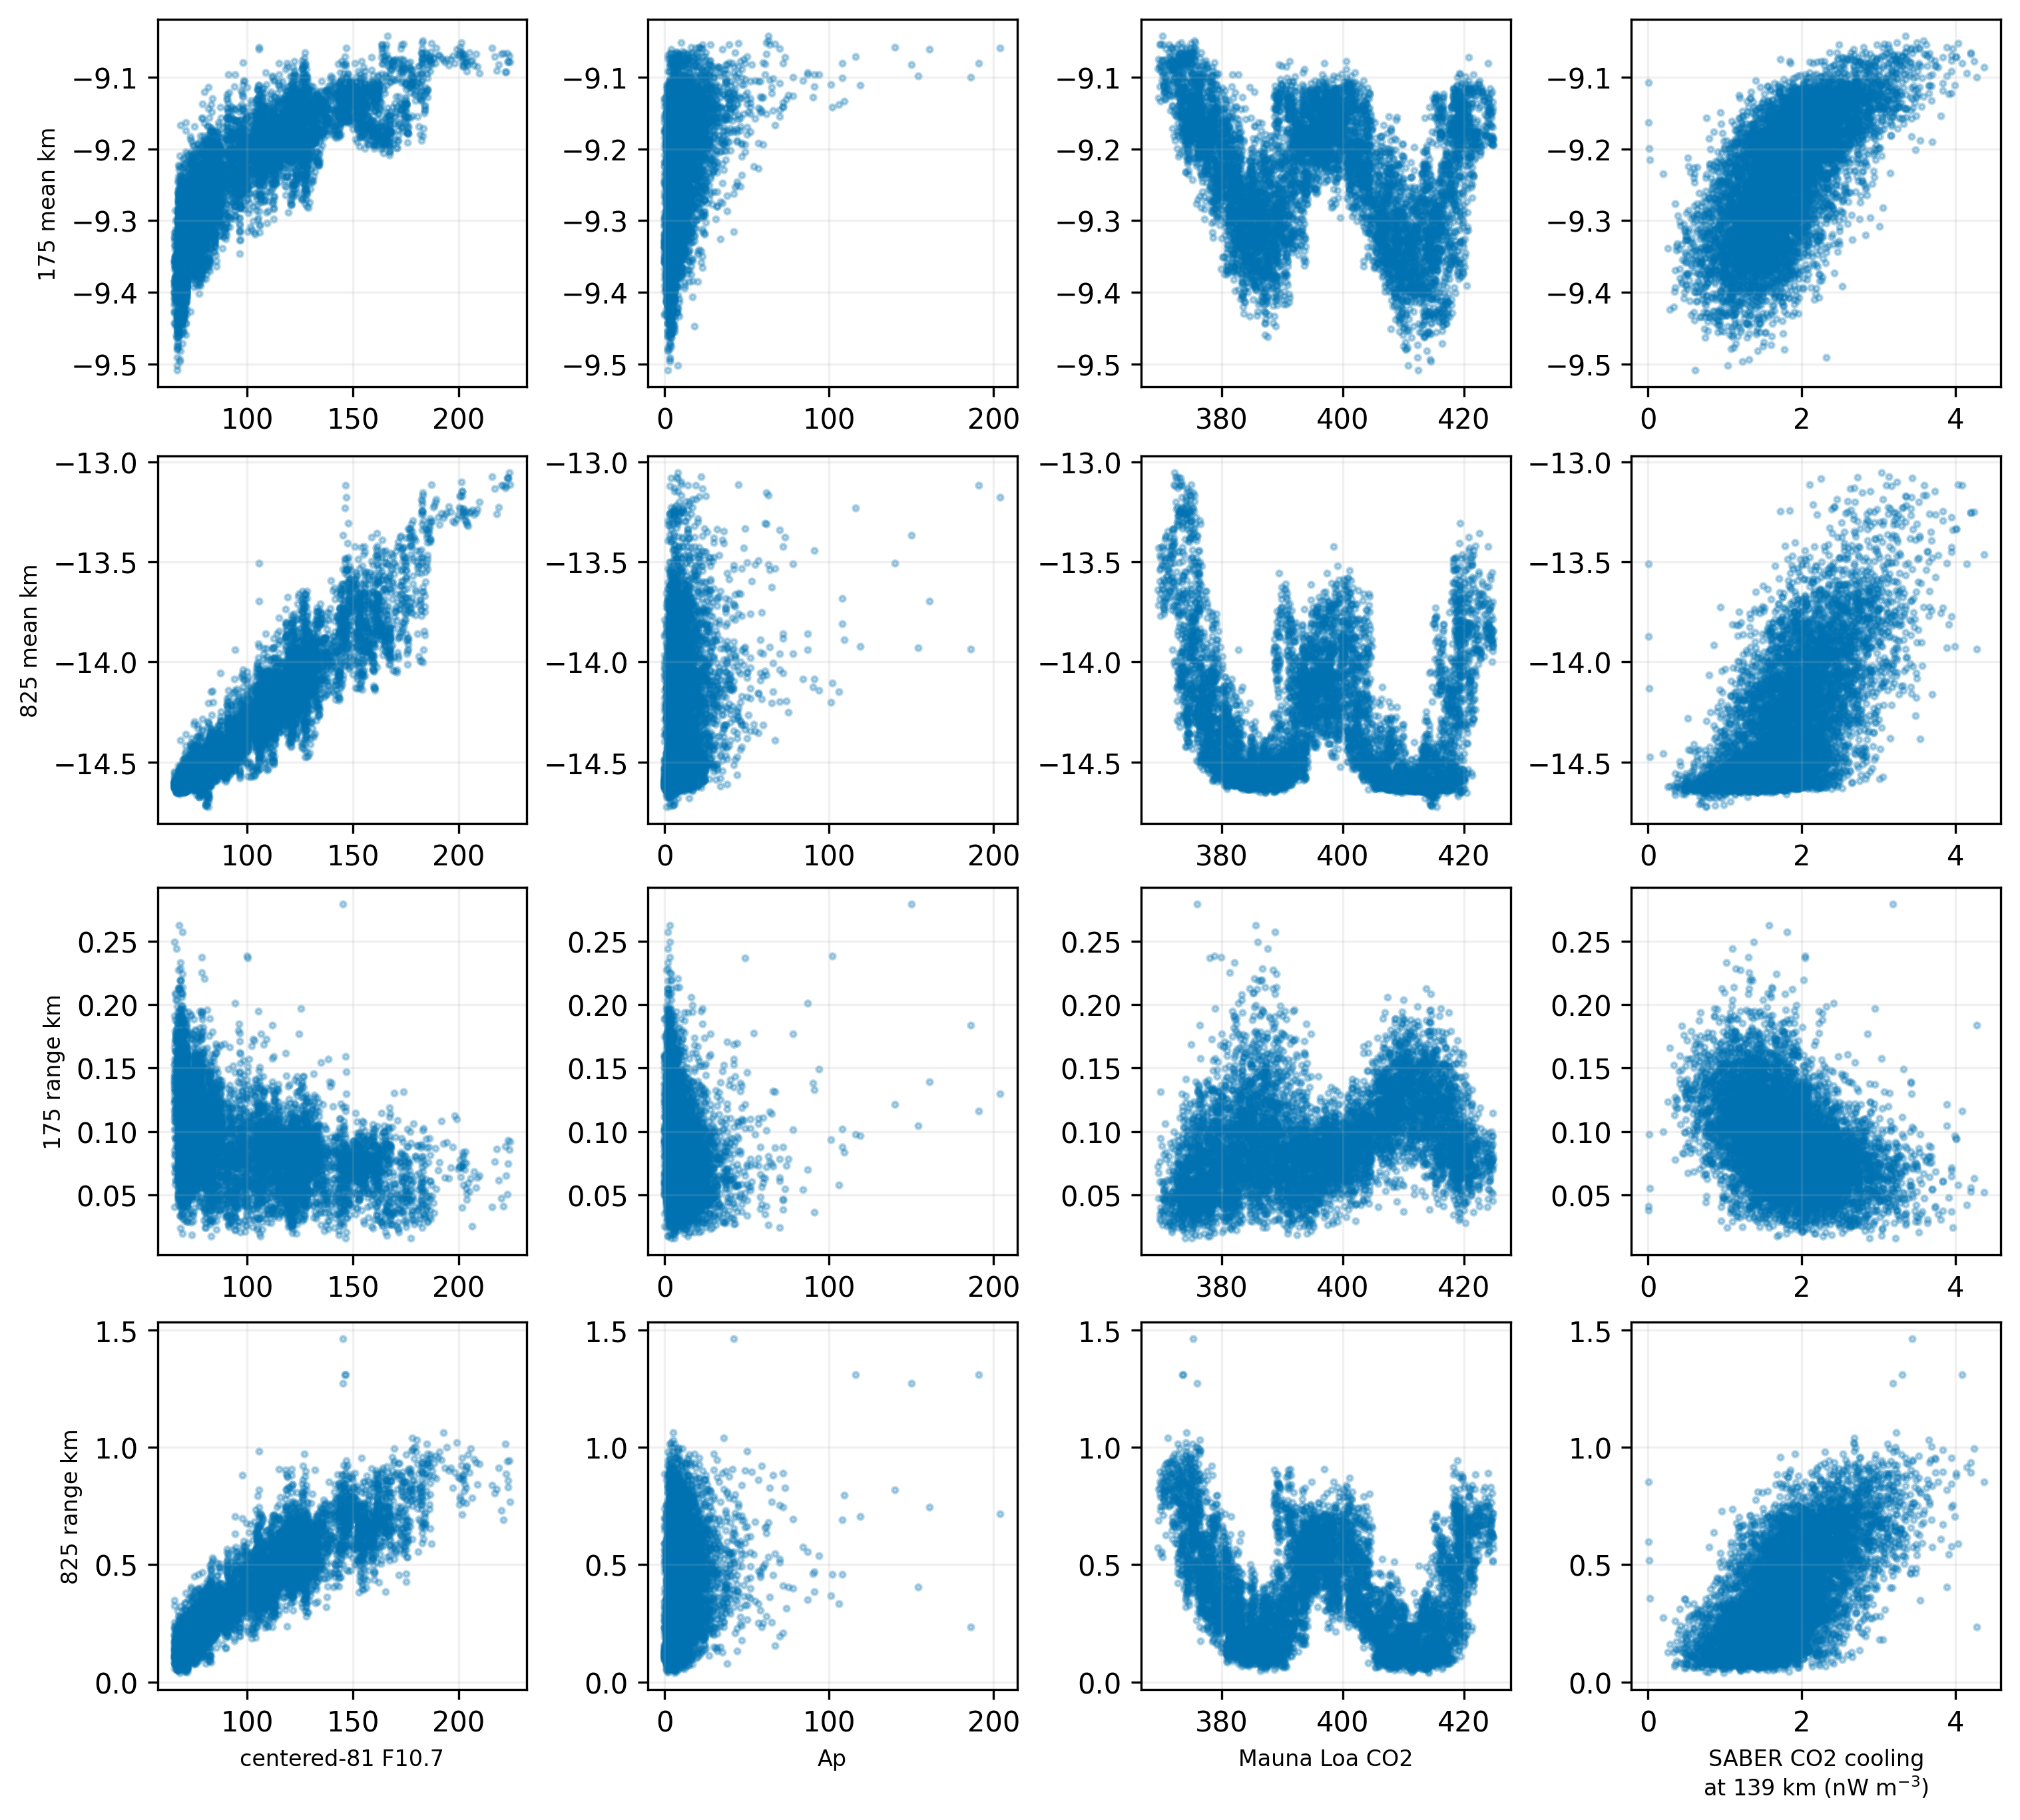
\includegraphics[width=0.95\textwidth]{fig3.pdf}
  \caption{Points-only descriptive scatter matrix.  Rows are HASDM daily mean
  log$_{10}$ density and within-day log-density range at 175 and 825 km; columns
  are centered-81-day F10.7, Ap, Mauna Loa CO$_2$, and SABER CO$_2$ cooling at
  139 km.  Pairwise missing values are omitted.}
  \label{fig:scatter}
\end{figure}

For the HASDM daily mean, altitude profiles remain strong for F10.7
($r=0.815$--$0.943$), moderate for SABER cooling ($r=0.656$--$0.664$), and
smaller for Kp ($r=0.337$--$0.458$) and Ap ($r=0.293$--$0.373$)
(Figure~\ref{fig:relationships}).  The CO$_2$ profile is consistently negative
($r=-0.260$ to $-0.132$).  In contrast, daily-range associations change sign
with altitude: F10.7 spans $-0.554$ to $0.899$, SABER cooling $-0.497$ to
$0.643$, Ap $-0.421$ to $0.219$, Kp $-0.558$ to $0.265$, and CO$_2$ $-0.229$
to $0.382$.  The smooth profiles partly arise because the altitude levels come
from one vertically coherent product.  The negative mean-density/CO$_2$
association is consistent in sign with long-term contraction, but a bivariate
correlation among trending, autocorrelated series cannot isolate radiative
forcing from solar-cycle sequencing, geomagnetic variability, or product
construction.

\begin{figure}[p]
  \centering
  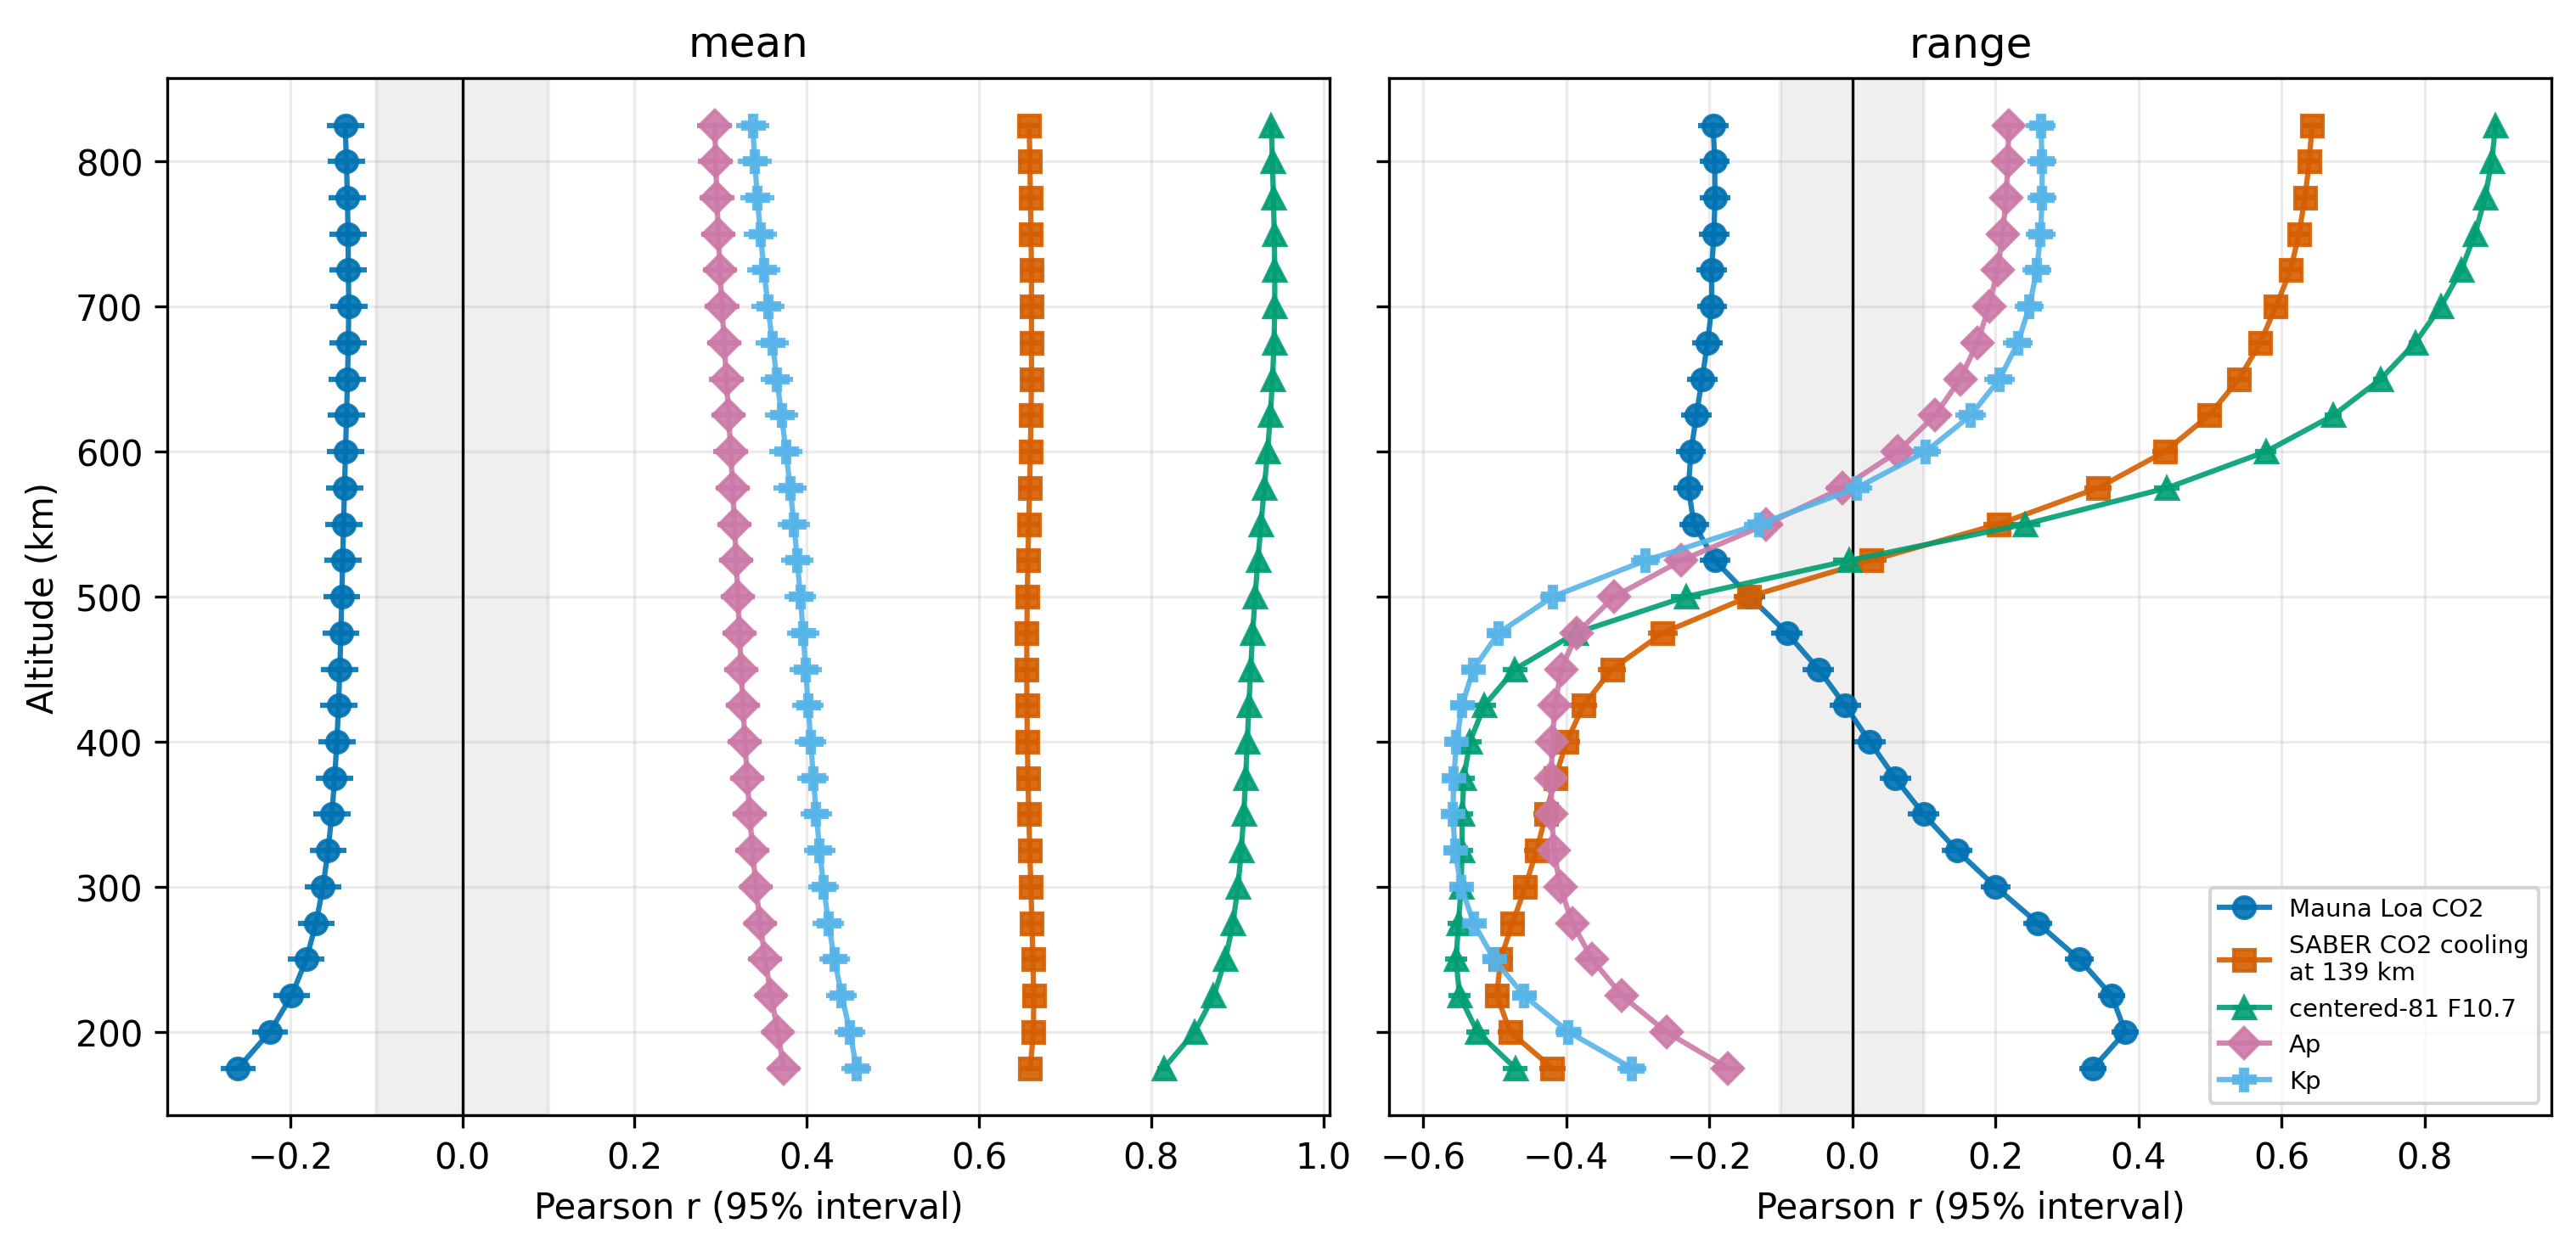
\includegraphics[width=\textwidth]{fig4.pdf}
  \caption{Altitude profiles of pairwise Pearson correlations for daily mean
  and range diagnostics with Mauna Loa CO$_2$, SABER cooling at 139 km, solar,
  and geomagnetic context.  Shading marks the near-zero reference band and
  horizontal bars are nominal Fisher 95\% intervals.  All associations are
  descriptive.}
  \label{fig:relationships}
\end{figure}

\subsection{Model accuracy and forcing fidelity are altitude dependent}

Across altitude, signed median errors range from $-0.061$ to $0.044$ for
JB2006, $-0.187$ to $-0.009$ for JB2008, $-0.117$ to $0.076$ for NRLMSISE-00,
and $-0.208$ to $-0.048$ for both NRLMSIS 2.0 and 2.1
(Figure~\ref{fig:model}).  Median absolute error ranges are 0.043--0.154,
0.040--0.190, 0.077--0.217, and 0.125--0.240, respectively.  Median values over
the 27 plotted altitudes are listed in Table~\ref{tab:model}.  These summaries
show conditional HASDM agreement, not a formal all-purpose ranking: the
reference is assimilative, calibration overlap differs, and operational
performance depends on epoch, location, activity, and error metric.

Centered-F10.7 residual links are retained at no altitude for JB2006 or JB2008
and at seven altitudes for each NRLMSIS-family model.  Ap residual links are
retained at 25 of 27 altitudes for JB2006 and all 27 for the other four models.
The signs and amplitudes vary; near-zero values do not prove forcing fidelity,
and widespread Ap links do not by themselves identify a missing causal process.
They show that model--HASDM disagreement retains forcing-organized structure
under this preprocessing and conditional-independence configuration.

\begin{table}[t]
\centering
\caption{Median empirical-model diagnostics over 27 altitudes on the exact
common sample.  Errors are natural-log density ratios.  Leakage medians can be
zero because no link was FDR retained at most altitudes.}
\label{tab:model}
\begin{tabular}{lrrrr}
\toprule
Model & Median bias & Median absolute error & F10.7 leakage & Ap leakage \\
\midrule
JB2006       & -0.017 & 0.121 & 0.000 &  0.118 \\
JB2008       & -0.125 & 0.142 & 0.000 &  0.198 \\
NRLMSISE-00  &  0.010 & 0.176 & 0.000 & -0.263 \\
NRLMSIS 2.0  & -0.104 & 0.202 & 0.000 & -0.260 \\
NRLMSIS 2.1  & -0.104 & 0.202 & 0.000 & -0.260 \\
\bottomrule
\end{tabular}
\end{table}

\begin{figure}[p]
  \centering
  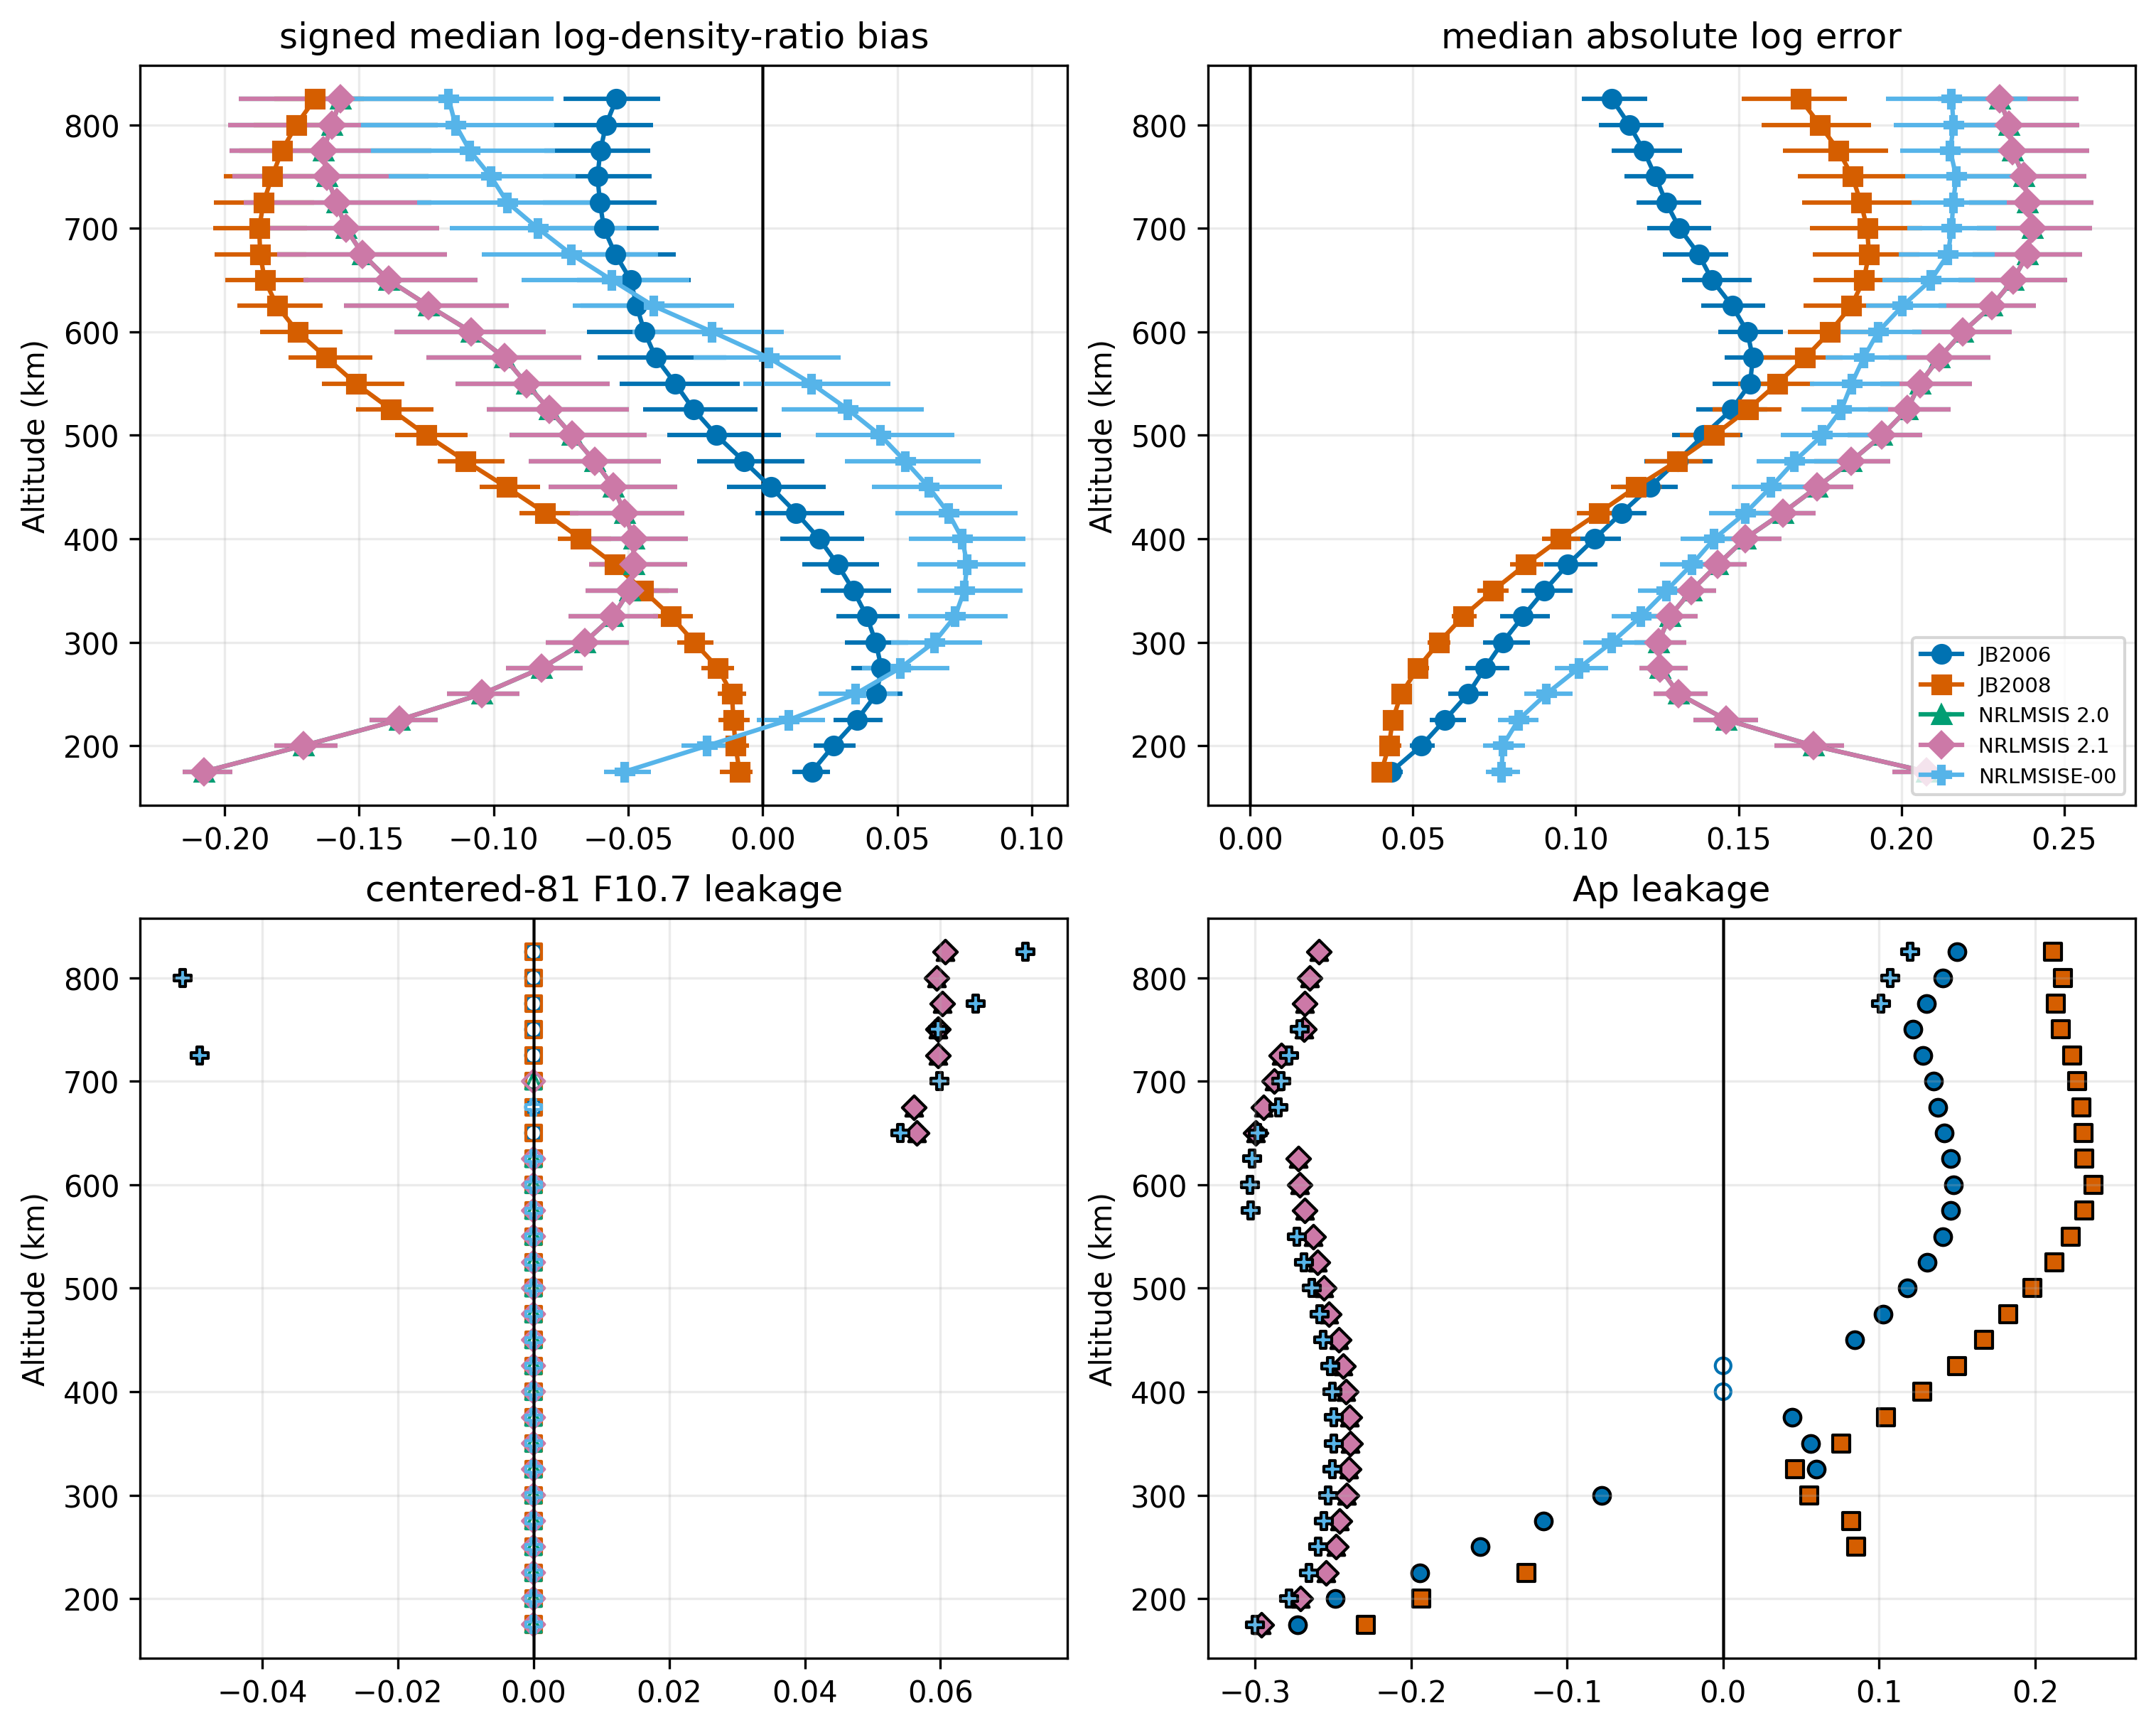
\includegraphics[width=0.95\textwidth]{fig5.pdf}
  \caption{On the exact common five-model sample, signed median log-density-ratio
  error and median absolute error are shown with precomputed 95\% paired
  circular-block-bootstrap intervals.  Centered-81-day F10.7 and Ap residual
  leakage panels use filled circles for FDR-retained links and open circles for
  non-retained links.  Zero means no retained link, not independence or a
  universal model ranking.}
  \label{fig:model}
\end{figure}

\subsection{Observed/reference and empirical-model trends diverge}

The reconstructed literature panel places most historical estimates between
$-7$ and $1\%$ decade$^{-1}$, with strong altitude and study dependence
(Figure~\ref{fig:trends}a).  Under the common quadratic-F10.7 adjustment, every
global-mean and HASDM point estimate is negative.  Global-mean estimates span
$-6.18$ to $-4.12\%$ decade$^{-1}$ (median $-5.04\%$), and HASDM estimates span
$-6.78$ to $-4.17\%$ decade$^{-1}$ (median $-6.36\%$).  The three retained TU
Delft altitude bins span $-3.16$ to $0.23\%$ decade$^{-1}$ (median $-1.21\%$),
with much shorter and mission-composite support.  Under this specified trend
model, all 10 global-mean and all 27 HASDM HAC intervals exclude zero on the
negative side; this does not substitute for alternative-model sensitivity.

The empirical baselines do not reproduce a common trend.  The three MSIS-family
profiles have median trends near $-1.3\%$ decade$^{-1}$, JB2006 has a median of
$-0.80\%$ decade$^{-1}$, and JB2008 has a median of
$-11.72\%$ decade$^{-1}$ (Table~\ref{tab:trends}).  NRLMSIS 2.0 and 2.1 are
nearly identical because the 2.1 change adds NO without refitting base mass
density.  JB2006 and JB2008 differ despite paired dates and locations, pointing
to their distinct proxy systems and formulations rather than an observed
climate contrast.  These model-generated slopes must not be pooled with
observational/reference slopes as independent estimates of thermospheric
contraction.

\begin{table}[t]
\centering
\caption{Solar-adjusted trend point-estimate ranges and medians over
product-specific retained altitudes.  Values are percent per decade;
uncertainty intervals appear in Figure~\ref{fig:trends}.}
\label{tab:trends}
\begin{tabular}{lrrrr}
\toprule
Dataset & $N_z$ & Minimum & Median & Maximum \\
\midrule
Global mean & 10 & -6.18 & -5.04 & -4.12 \\
Mauna Loa HASDM subset & 27 & -6.78 & -6.36 & -4.17 \\
TU Delft satellite density & 3 & -3.16 & -1.21 & 0.23 \\
NRLMSISE-00 baseline & 29 & -1.82 & -1.33 & -0.08 \\
NRLMSIS 2.0 baseline & 29 & -1.77 & -1.28 & -0.09 \\
NRLMSIS 2.1 baseline & 29 & -1.77 & -1.28 & -0.09 \\
JB2006 baseline & 29 & -1.26 & -0.80 & 0.04 \\
JB2008 baseline & 29 & -13.84 & -11.72 & -0.14 \\
\bottomrule
\end{tabular}
\end{table}

\begin{figure}[p]
  \centering
  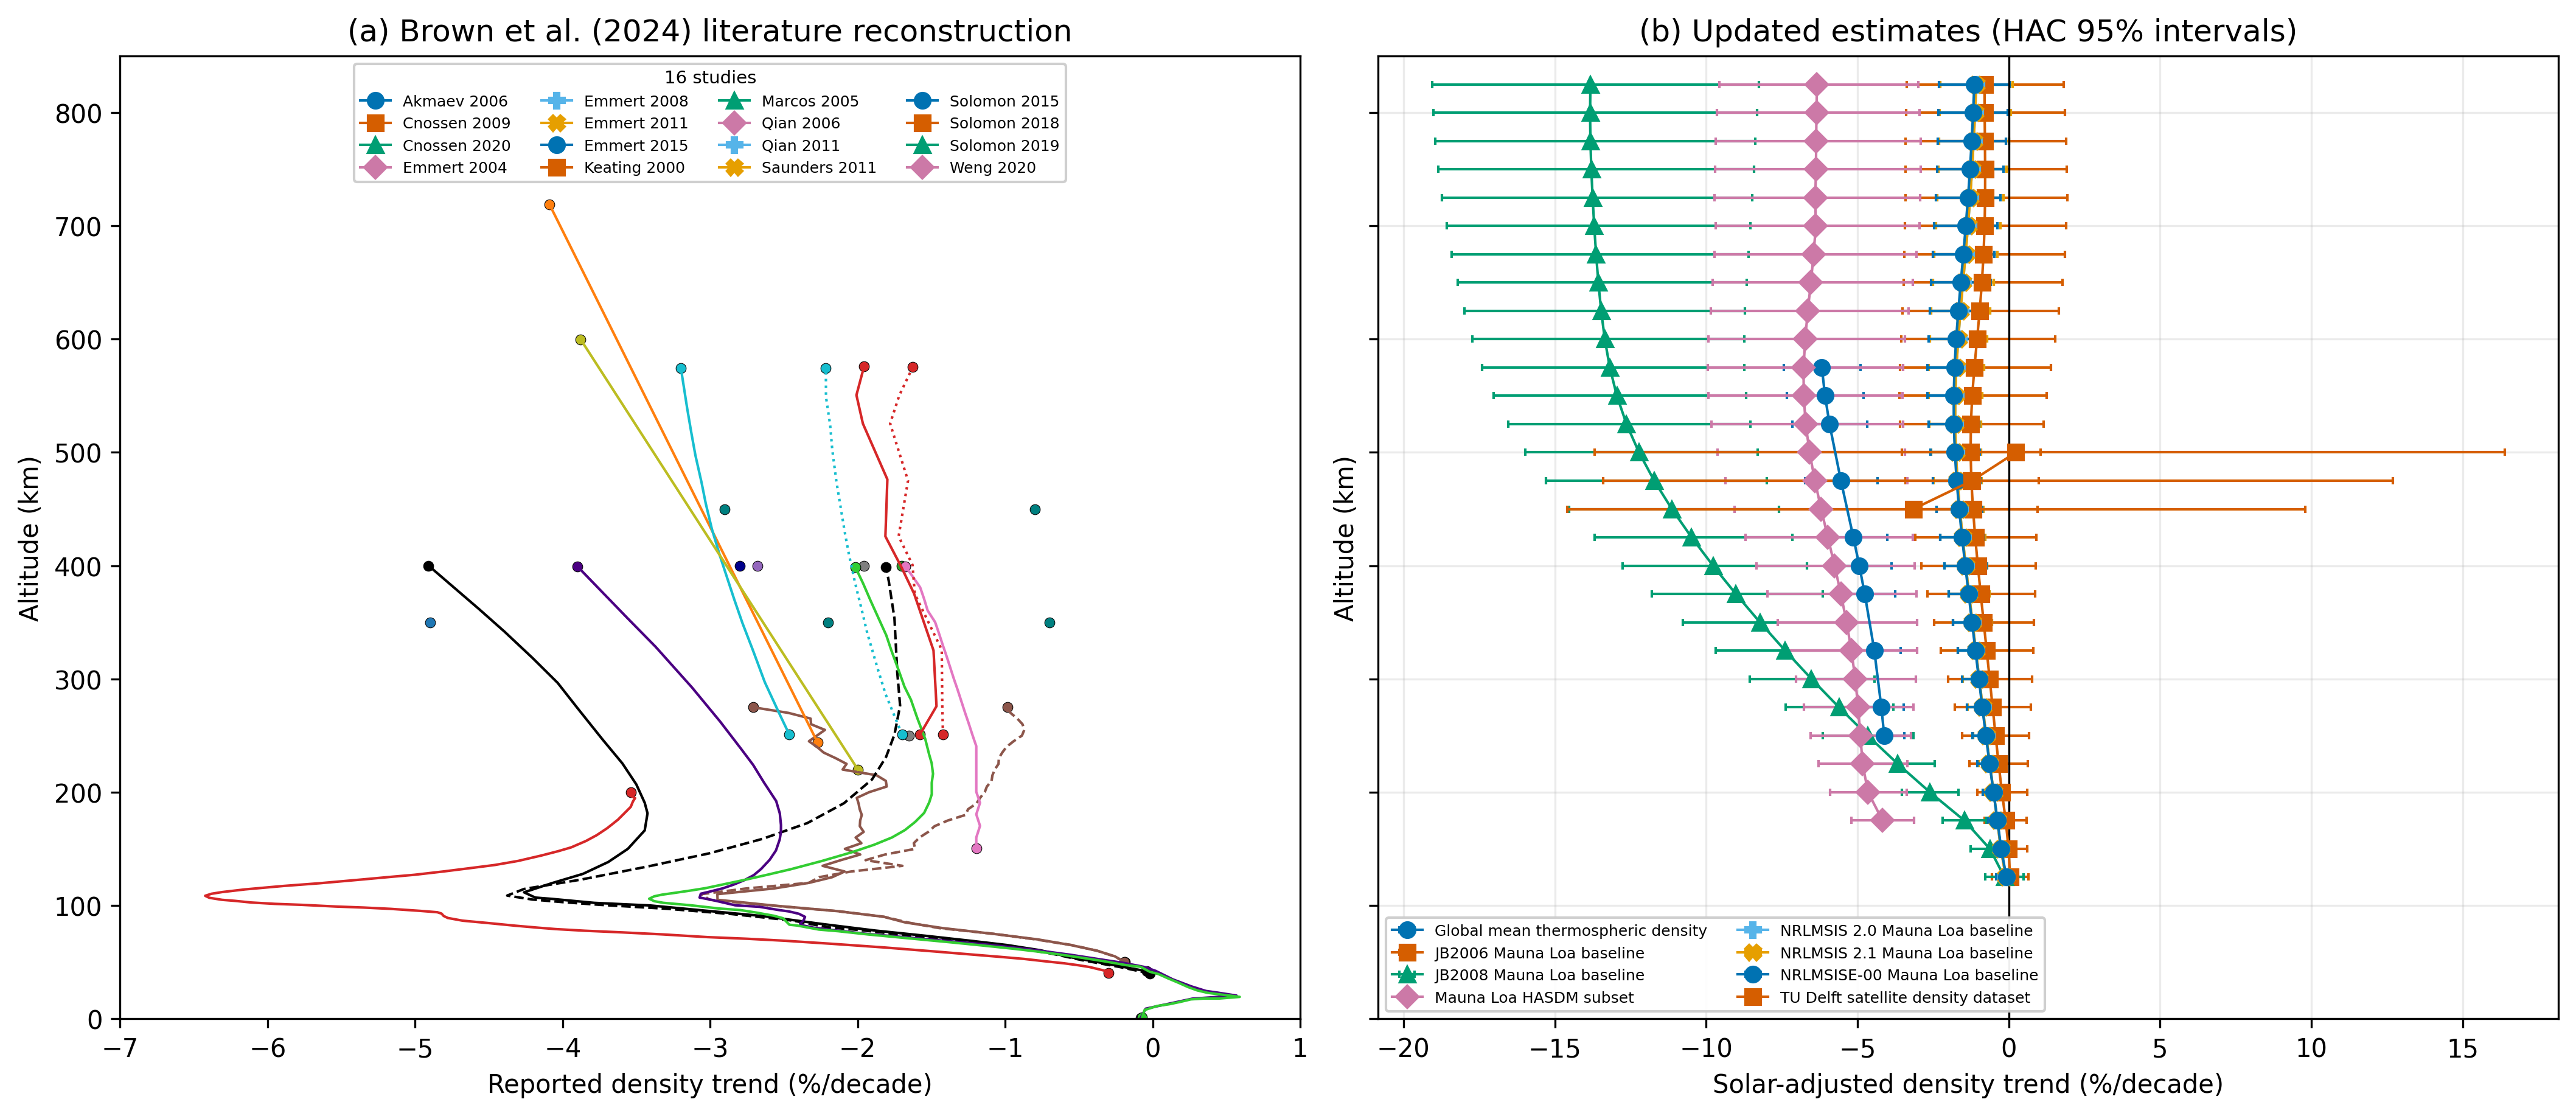
\includegraphics[width=\textwidth]{fig6.pdf}
  \caption{Density-trend synthesis.  (a) Vector rendering of plot-precision
  values digitized from \citet{brown2024} Figure~2 under CC BY 4.0; these are
  not replacement study data.  (b) Solar-adjusted log$_{10}$-density trends
  with 27-day HAC 95\% intervals, including paired JB2006/JB2008.  Trends are
  descriptive and method- and sampling-dependent, not CO$_2$-only estimates.}
  \label{fig:trends}
\end{figure}

\section{Discussion}

\subsection{A consistent hierarchy of variability, but not of attribution}

The cross-product comparison yields a robust first-order result: centered
81-day solar activity strongly organizes mean thermospheric density.  The
result appears in the global-mean and HASDM products and is intentionally
recovered by all five empirical models.  Geomagnetic correlations are smaller
for daily means but remain substantial, while daily ranges contain pronounced
altitude-dependent sign changes.  Those range profiles are useful diagnostics
of variability represented by each product, but they should not be read as
simple thermodynamic transfer functions.

SABER CO$_2$ cooling covaries positively with HASDM mean density.  This
association may reflect shared solar-cycle variability, but the bivariate
analysis cannot establish that mechanism.  Tropospheric CO$_2$
covaries negatively with mean density because it increases over the same epoch
in which secular contraction is expected.  These opposite bivariate signs are
not contradictory: one quantity is a radiative-cooling response that varies
strongly with current thermospheric energy input, whereas the other is a
slowly varying lower-atmosphere concentration.  Neither correlation estimates
the causal effect of increasing CO$_2$.  Attribution would require an explicit
physical or statistical identification strategy, sensitivity to alternative
solar and geomagnetic controls, and a model for the shared nonstationarity.

\subsection{Residual leakage complements, rather than replaces, accuracy}

Figure~\ref{fig:model} separates the size of model disagreement from its
forcing organization.  A model can have a relatively small median absolute
error while retaining Ap-structured residuals, or a larger absolute error with
little retained centered-F10.7 structure.  Because HASDM itself assimilates
drag information and empirical models were calibrated on different but partly
overlapping domains, the residuals do not compare five independent forecasts
against ground truth.  The paired design removes sample-composition differences
within the plotted comparison, but it cannot remove calibration overlap or
reference error.

The absence of retained centered-F10.7 links for the JB pair is therefore not
proof that their solar forcing is optimal.  Their solar proxies differ from the
single displayed centered F10.7 series, and the maximum-retained-lag summary is
sensitive to preprocessing, lag window, and multiplicity control.  Conversely,
the widespread Ap links deserve model-development attention but not a causal
label.  Independent tests at trajectory locations and held-out epochs are the
appropriate next step.

\subsection{Trend disagreement is itself an operational result}

The global-mean and HASDM trend profiles both yield negative point estimates
of several percent per decade after the same solar adjustment, broadly consistent with
the historical literature synthesis.  Their difference is plausible given
their disjoint spatial definitions, epochs, altitudes, and construction.
The much shorter TU Delft trend support explains its sparse and less stable
profile.

The empirical baselines reveal a separate point.  A long model-generated record
is not automatically a neutral climate baseline.  If proxy series, lag
conventions, validity windows, or internal climatologies drift differently,
the fitted calendar coefficient can differ dramatically even on paired dates
and locations.  The JB2008 profile is the clearest example.  It should be
interpreted as the trend produced by that executable model and its retrieved
drivers, not as evidence for exceptionally rapid atmospheric contraction.
Likewise, the near-identical NRLMSIS 2.0 and 2.1 profiles are a formulation
consequence, not independent replication.

\subsection{Limitations}

Several limitations bound the claims.  First, products differ in geography,
sampling, calibration, and assimilation; Figure~\ref{fig:coverage} does not
make them commensurate.  Second, Fisher correlation intervals are nominal under
daily autocorrelation.  Third, the relationship figures are pairwise and do not
adjust for shared seasonality or trends.  Fourth, the HASDM analysis uses one
geographic vertical subset, and it is not an in situ truth standard.  Fifth,
the trend regression removes a quadratic F10.7 response but not every possible
solar, geomagnetic, seasonal, compositional, or instrumental confounder.  Sixth,
the model-error leakage analysis is exploratory and collapses a lag graph into
one retained effect per forcing and altitude.  Finally, F30, SABER NO cooling,
and hmF2/NmF2 extensions were not locally analysis-ready and were deliberately
deferred rather than represented by placeholders.

\section{Conclusions}

\begin{enumerate}
  \item Mean thermospheric density has a strong positive centered-81-day F10.7
  response across observational/reference products and all five empirical
  baselines, but response strength remains altitude and product dependent.
  \item HASDM mean density is positively associated with SABER CO$_2$ cooling
  and geomagnetic activity and negatively associated with tropospheric CO$_2$;
  these bivariate relationships are descriptive and do not identify a CO$_2$
  causal effect.
  \item Exact-common-sample model errors and residual leakage supply different
  information.  Both vary with altitude, and calibration overlap prevents a
  universal independent model ranking.
  \item Common solar-adjusted regressions yield median negative trends near
  $-5.0\%$ decade$^{-1}$ in the global-mean record and $-6.4\%$ decade$^{-1}$
  in the Mauna Loa HASDM subset.
  \item Large disagreement among empirical-baseline trends---especially the
  paired JB2006/JB2008 contrast---shows that model-generated trend profiles are
  forcing- and formulation-dependent diagnostics, not interchangeable climate
  observations.
\end{enumerate}

\section*{Open research and reproducibility}

The analysis code, figure builder, tests, manuscript source, captions, alt text,
and machine-readable source checksums are maintained in the Thermodense
repository at \url{https://github.com/Sergiogd112/thermodense}.  The six figures
can be regenerated from prepared artifacts with
\texttt{scripts/build\_first\_paper\_figures.py}.  Some inputs require provider
access or carry redistribution restrictions; consequently the repository
documents access routes and provenance rather than redistributing all source
data or JB provider software.  Figure~\ref{fig:trends}a is redistributed as a
new vector rendering from attributed CC BY 4.0 plot-precision data.

\section*{Acknowledgments}

The author acknowledges the U.S. Naval Research Laboratory and CEDAR data
services for the global-mean density product, Space Environment Technologies
for HASDM and JB resources, TU Delft for version-02 thermospheric density data,
NOAA Global Monitoring Laboratory for Mauna Loa CO$_2$, the TIMED/SABER team for
cooling-rate observations, and the providers of the solar and geomagnetic
indices.  Provider acknowledgment does not imply endorsement of the analysis.

\section*{Competing interests}
The author declares no competing interests.

\bibliographystyle{plainnat}
\bibliography{references}

\end{document}
